\documentclass[journal]{IEEEtran}

\usepackage{blindtext}
\usepackage{cite}
\usepackage{graphicx}
\usepackage{array}
\usepackage{color}
\usepackage{tabularx}
\usepackage{epsfig}
\usepackage{amsmath}
\usepackage{amssymb}
\usepackage{bm}
\usepackage{wasysym}
\usepackage{circuitikz}
\usepackage{float}
\usepackage{algorithm}
\usepackage{algorithmic}

\usetikzlibrary{arrows,shapes,calc,positioning}

\newcommand{\myscope}[2]
{\draw[thick,rotate=#2] (#1) circle (12pt)
(#1) ++(-0.35,-0.1) --++ (0.3,0.3) --++ (0,-0.3) --++(0.3,0.3) --++(0,-0.3);}

\begin{document}

\title{CSCE 221 \\ Problem Set 12}

\author{Jacob~Purcell,~\IEEEmember{Texas~A\&M,~Student}}

\maketitle
\section{}

Deletion in a redblack tree goes as,

\begin{algorithm}
    \caption{Void Delete}
    \begin{algorithmic}
        \REQUIRE $Red~Black~Tree$
        \STATE $Pointer~C~=~Find~X$
        \IF{$both~of~C~children~are~nullptr$}
        \STATE $Delete C$
        \ENDIF


        \STATE $Pointer~B~=~C~left~child$
        \WHILE{$B~right~child~is~not~nullptr$}
        \STATE $Assign~B~to~be~its~right~child$
        \ENDWHILE
        \STATE $set~value~at~C~to~be~B$
        \STATE $C~takes~over~right~subtree~of~B~if~needed$
        \STATE $delete~B$
        \STATE $Flip~colors~of~C~and~children$
        \STATE $Rotate~unbalanced~nodes~to~maintain~the~4th~rule$
        
    \end{algorithmic}
\end{algorithm}

\section{}
To get the maximum height, we qill use
$$N_h = N_r + N_b$$
which states that the height is determined by the maximum number of red and black nodes allowable per the rules of Red Black Trees.
In an AVL tree, it is known that the total number of nodes is 

$$N = 2^{h+1}-1$$

Solving for the height plus 1(k) to account for the root node,

$$k = log(N+1)$$

this number represents the total number of nodes in the longest subtree of an AVL Tree, 
but since in a Red Black Tree only black nodes are counted, the longest subtree may be doubled to give the total number of nodes,

$$N_h = \boxed{2log(N+1)}$$

\section{}

Figure 1 is shown with a balance of $0$ which meets the requirements of an AVL Tree while also being a Red Black Tree.
The root node in Figure 2 has a balance of 2 which violates the balance condition for an AVL Tree, however, this tree still fulfills 
all of the necessary conditions for a Red Black Tree.

\begin{figure}[h!]
    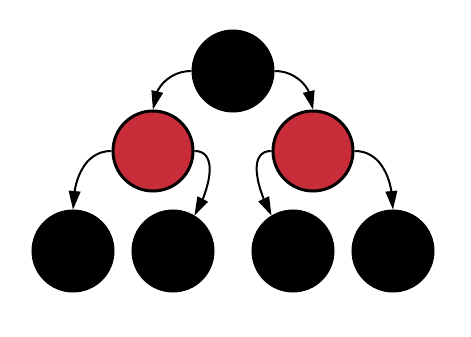
\includegraphics[scale = 0.5]{p1.png}
    \caption{AVL balanced Red Black Tree.}
\end{figure}
\begin{figure}[h!]
    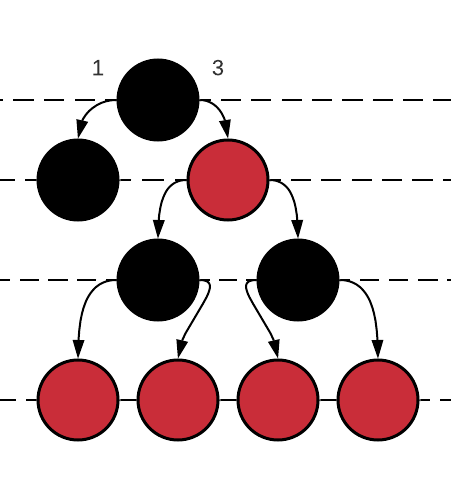
\includegraphics[scale = 0.5]{p2.png}
    \caption{Non-AVL Red Black Tree.}
\end{figure}


\end{document}
